%%%%%%%%%%%%%%%
%							TEST MODEL 
%%%%%%%%%%%%%%%

\subsection{Project Test Model} \label{section:project-model}

\paragraph{}
This section outlines the test model that was created after the draft model stage, QUT data access and initial photovoltaic systems analysis. In order to create the test model of a ``real-world" Brisbane based commercial building to structure the analysis around, the QUT schematics and personal experience within Brisbane's built environment were integral. 

\subsubsection{Lighting Loads}

\paragraph{}
To calculate approximate lighting loads to be expected for a floor, level 7 of QUT P Block was marked up to count the number of luminaires installed. A full floor plan is shown in Appendix \ref{appendix:qut_lvl6_markup} but an image export is below in Figure \ref{fig:qut-lvl6-lighting-markup}.      

\begin{figure}[H]
	\hfill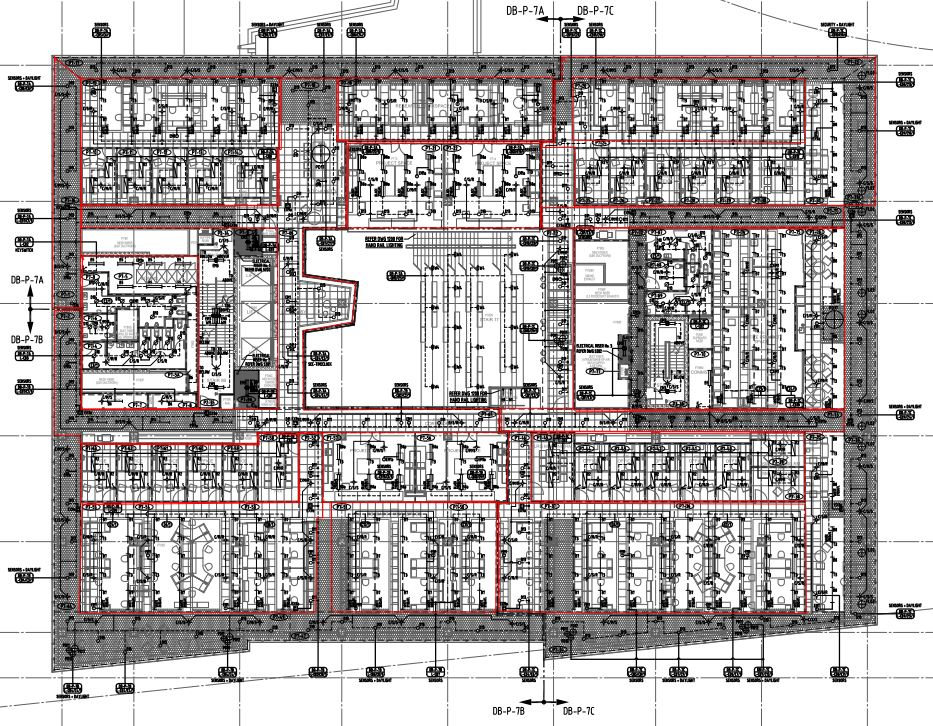
\includegraphics[width = 150mm]{images/project-model/qut-lvl7-lighting-markup}\hspace*{\fill}
	\caption{QUT: P Block Level 6 Lighting Markup} 
	\label{fig:qut-lvl6-lighting-markup}
\end{figure}

\paragraph{}
Table \ref{table:QUTlvl7-count} below outlines the counts from the markup. These were then used to calculate total loads for the floor plan. With these values, a test model can be based with an approximate light load that can be separated over dedicated DC distribution boards over the floor once further calculations and photovoltaics layouts are designed. This model will be utilised in Section \ref{section:project-questions} for deep analysis and simulation. This is the reasoning behind utilising the QUT provided floor plans to attempt to create an accurate ``real world" example of DC distribution implementation.     

\begin{table}[!ht]
	\centering
	\renewcommand{\arraystretch}{2}
	\begin{tabular}{|c|c|c|c|c|}
		\hline
		\textbf{Fitting} & \textbf{Wattage (W)} & \textbf{Voltage (V)} & \textbf{Count} & \textbf{Demand (A)} \\ \hline
		LED Downlight & 36.0 & 24.0 & 110.0 & 165.0 \\ \hline
		LED Barlight & 56.0 & 24.0 & 224.0 & 522.7 \\ \hline
	\end{tabular}

	\caption{QUT: P Block Level 7 Lighting Count and Calculations}
	\label{table:QUTlvl7-count}
\end{table}

\subsubsection{Floor Size}

\paragraph{}
The same floor plan layout was loaded into AutoCad to calculate the area and average room size. The entire floor plan was measure to be approximate 65\,m by 47\,m providing an area of approximately 3000\,\si{m^2}. The average office size of 22\,\si{m^2}. 

\subsubsection{Photovoltaic Modules}

\paragraph{}
This information is elaborated on further in Section \ref{section:PV-panels} however to briefly preface, the test model will be based on utilising the average photovoltaic module of 265\,W of assumed size 1600\,mm by 1000\,mm by 35\,mm. This value will be used in analysisng PV quantities with available spacings as well as power production simulation with System Advisor Model. 

\subsubsection{Electrical Infrastructure}

\paragraph{}
The assumption for this project is that separate DC electrical infrastructure will be installed to power the chosen devices. At this stage, devices cannot be selected because loads have to be analysed first after photovoltaic modelling. Ideally, reputable brands for electrical equipment such as Eaton or NHP will be selected with preference to affordable but safe models. Eaton products are generally more affordable and will likely be chosen for the switchboards and circuit breakers. Additionally, it is generally far easier to alter settings to remove faults when the same manufacturer is used for the complete circuits.  

\subsubsection{Photovoltaic Mounting}

\paragraph{Fixed Mounted} 
~\\
There are multiple options for fixing modules to the selected surface areas and each has their own merit. The most popular solution are frames specifically designed to mount an array of panels on a roof, ground or other surface and keep them still in place. This is known as a fixed mounting scheme \cite{Haberlin2012}. Clips or conventional screws can be used to mount the modules to these frames. Two examples of this mounting scheme is shown in Figure \ref{fig:pv-mounting-fixed-field} and Figure \ref{fig:pv-mounting-fixed-roof}. 

\begin{figure}[H]
	\hfill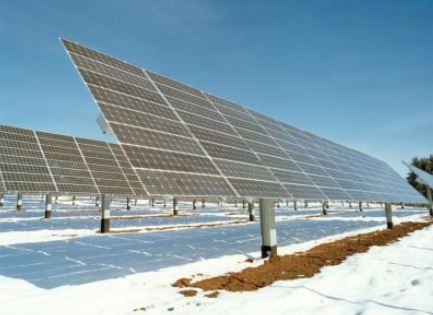
\includegraphics[width = 100mm]{images/pv-fixed-mounting}\hspace*{\fill}
	\caption{Fixed Mounted Photovoltatic System \cite{Haberlin2012}} 
	\label{fig:pv-mounting-fixed-field}
\end{figure}

\begin{figure}[H]
	\hfill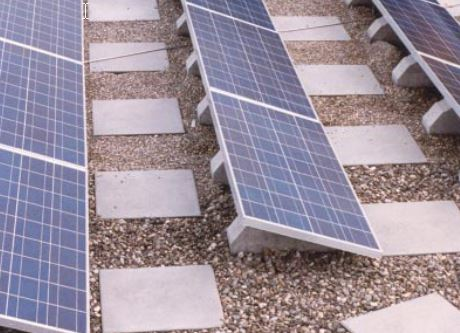
\includegraphics[width = 100mm]{images/pv-roof-mounting}\hspace*{\fill}
	\caption{Roof Mounted Photovoltatic System \cite{Haberlin2012}} 
	\label{fig:pv-mounting-fixed-roof}
\end{figure}  

\paragraph{Building Integration Mounting}
~\\
There also exists creative solutions to mounting photovoltaic modules. This can be replacing roof material with modules or using them as window awnings. An example of this from the US Embassy in Geveva is shown in Figure \ref{fig:pv-mounting-fixed-windows}.  
	
\begin{figure}[H]
	\hfill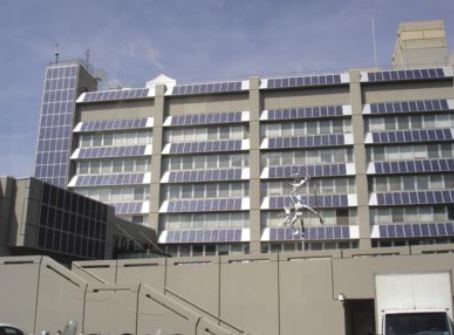
\includegraphics[width = 100mm]{images/pv-mouting-windows}\hspace*{\fill}
	\caption{Window Awning Mounted Photovoltatic System \cite{Haberlin2012}} 
	\label{fig:pv-mounting-fixed-windows}
\end{figure} 

\paragraph{Single and Dual Axis Tracking System}
~\\
The yield of modules can be increased by implementing tracking systems in the modules' installations. These can be single or dual axis tracking systems. Single axis, as the name suggests, means that it will shift in one direction, back and forward, traditionally on a timer. The idea behind these is that as the day progresses, the module is able to shift to continually face the sun and receive the maximum luminance in order to increase production \cite{Haberlin2012}. An examle of this installation is shown in Figure \ref{fig:pv-mounting-single-axis}. Dual axis, again as the name suggests, shifts the module across two axes for even further increased production from the installed modules. These systems of course both require power to operate so it is possible to have a higher production than fixed axis however net production after operating the control systems could be lower.  

\begin{figure}[H]
	\hfill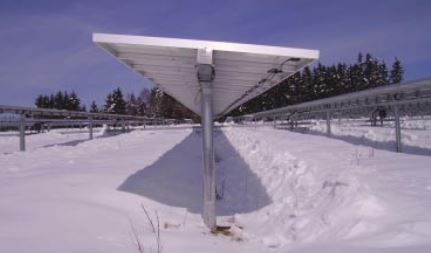
\includegraphics[width = 100mm]{images/pv-mouting-rotating}\hspace*{\fill}
	\caption{Single Axes Mounting \cite{Haberlin2012}} 
	\label{fig:pv-mounting-single-axis}
\end{figure} 
       
  
 